\documentclass[sigconf,nonacm]{acmart}

\settopmatter{printacmref=false}
\setcopyright{none}
\usepackage{booktabs}
\usepackage{graphicx}

\title{Predicting Concrete Compressive Strength with a Multilayer Perceptron}

\begin{document}
\begin{abstract}
This study predicts concrete compressive strength from mixture proportions and curing age using the UCI Concrete Compressive Strength dataset. A multilayer perceptron (MLP) is compared with linear regression, followed by five one-factor configurations evaluated with three training seeds. CPU and GPU training times are also measured. On a fixed test split, the baseline MLP obtains an RMSE of 6.893 MPa, compared with 11.002 MPa for linear regression. Among the tested configurations, a learning rate of 0.01 gives the lowest mean test RMSE (6.398 MPa). For this small network on the available computer, CPU training is faster than GPU training. These results illustrate the value of nonlinear models and controlled comparisons, while also showing that findings depend on the split, model size, and hardware.
\end{abstract}

\maketitle

\section{Introduction}
Concrete strength depends on interacting mixture components and curing age. Predicting strength from these measurements is a regression task: the model returns a continuous value in megapascals (MPa). This project asks whether a small neural network improves on a linear baseline, how selected training choices affect prediction, and whether GPU execution reduces training time for this workload.

\section{Data and Methods}
\subsection{Dataset and preprocessing}
The UCI dataset contains 1,030 observations, eight quantitative input features, and one strength target, with no missing values reported \cite{uci,yeh}. Inputs are cement, blast furnace slag, fly ash, water, superplasticizer, coarse aggregate, fine aggregate (all in kg/m$^3$), and age (days). The target is concrete compressive strength in MPa.

A fixed random split (seed 42) assigns 60\% of observations to training and 20\% each to validation and test (618/206/206). Inputs are standardized using means and standard deviations fitted only on the training split, preventing information from validation and test data from entering preprocessing. The target remains in MPa. The test split is held fixed across the compared configurations.

\subsection{Models and training}
The linear regression model is the reference baseline. The MLP maps eight inputs through fully connected layers with ReLU activations, using architecture $8\rightarrow32\rightarrow16\rightarrow1$. It is trained with Adam, a 0.001 learning rate, batch size 32, mean squared error loss, and at most 300 epochs. The checkpoint with the lowest validation RMSE is selected. MAE and RMSE are reported in MPa; R$^2$ summarizes explained variation, with larger values generally preferred.

For the ablation study, training seeds 42, 43, and 44 control initialization and batch order, while the data split stays fixed. Five configurations are compared: baseline; no input standardization; one hidden layer ($8\rightarrow32\rightarrow1$); a narrower network ($8\rightarrow16\rightarrow8\rightarrow1$); and learning rate 0.01. Each changes one factor relative to baseline. The best epoch is selected by validation RMSE, and test metrics are then computed for comparison.

\section{Experimental Results}
\subsection{Linear baseline and MLP}
Table~\ref{tab:baseline} answers whether the nonlinear model improves on a simple linear mapping under the same split. The MLP reduces test RMSE from 11.002 to 6.893 MPa and MAE from 8.488 to 5.309 MPa, while R$^2$ rises from 0.585 to 0.837. This indicates that the MLP captures useful nonlinear relationships in the mixture data, although it does not establish that neural networks will always outperform linear models on other splits.

\begin{table}[t]
\caption{Baseline performance on the fixed test split.}
\label{tab:baseline}
\centering
\small
\begin{tabular}{lrrr}
\toprule
Model & MAE (MPa) & RMSE (MPa) & R$^2$\\
\midrule
Linear regression & 8.488 & 11.002 & 0.585\\
MLP (8-32-16-1) & 5.309 & 6.893 & 0.837\\
\bottomrule
\end{tabular}
\end{table}

Figure~\ref{fig:training} shows the baseline learning curves. Training and validation RMSE fall substantially from their initial values. The best validation RMSE is 6.385 MPa at epoch 292; the close training and validation trajectories late in training provide no strong visual evidence of a widening generalization gap in this run.

\begin{figure}[t]
\centering
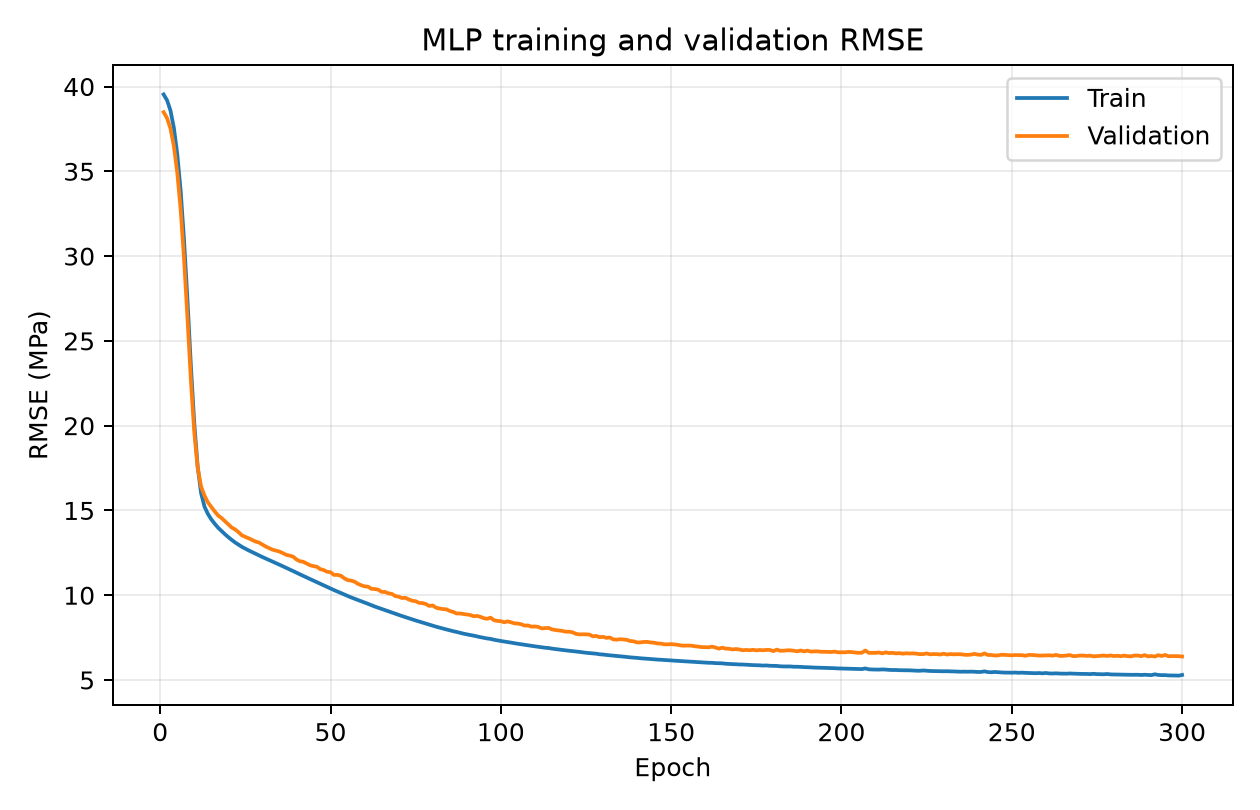
\includegraphics[width=\columnwidth]{images/training_curve.png}
\caption{Baseline MLP training and validation RMSE across epochs.}
\Description{A line chart showing train and validation RMSE decreasing rapidly at first and then gradually leveling off over 300 epochs.}
\label{fig:training}
\end{figure}

\begin{table*}[t]
\caption{Five MLP configurations. Values are mean $\pm$ standard deviation over seeds 42, 43, and 44; validation RMSE is taken at each seed's selected epoch.}
\label{tab:ablation}
\centering
\small
\begin{tabular}{lrrrr}
\toprule
Configuration & Validation RMSE (MPa) & Test MAE (MPa) & Test RMSE (MPa) & Test R$^2$\\
\midrule
Baseline (8-32-16-1) & 6.003 $\pm$ 0.334 & 5.260 $\pm$ 0.136 & 6.870 $\pm$ 0.054 & 0.838 $\pm$ 0.003\\
No standardization & 6.061 $\pm$ 0.217 & 5.358 $\pm$ 0.199 & 7.103 $\pm$ 0.205 & 0.827 $\pm$ 0.010\\
One hidden layer (8-32-1) & 8.569 $\pm$ 1.747 & 7.113 $\pm$ 1.279 & 9.121 $\pm$ 1.516 & 0.709 $\pm$ 0.098\\
Narrow (8-16-8-1) & 8.414 $\pm$ 1.872 & 7.010 $\pm$ 1.266 & 9.115 $\pm$ 1.453 & 0.710 $\pm$ 0.093\\
Learning rate 0.01 & 5.151 $\pm$ 0.250 & 4.680 $\pm$ 0.472 & 6.398 $\pm$ 0.452 & 0.859 $\pm$ 0.020\\
\bottomrule
\end{tabular}
\end{table*}

\begin{figure*}[t]
\centering
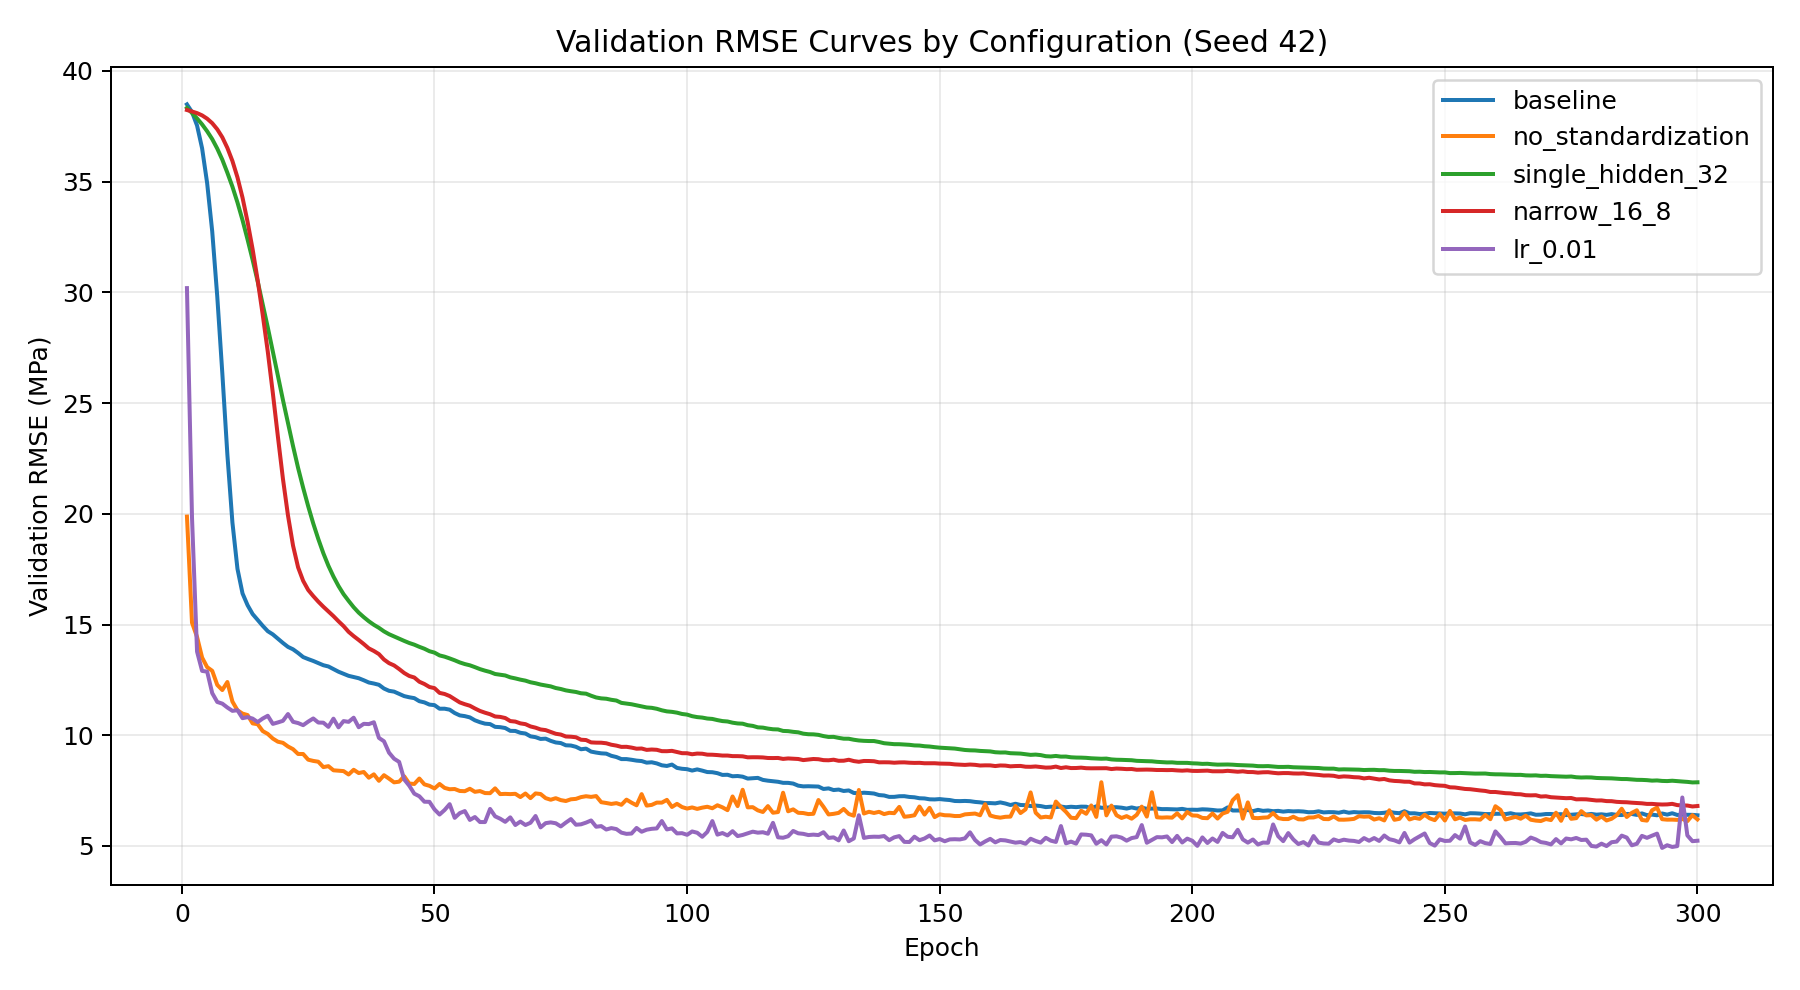
\includegraphics[width=0.485\textwidth]{images/ablation_val_curves_seed42.png}
\hfill
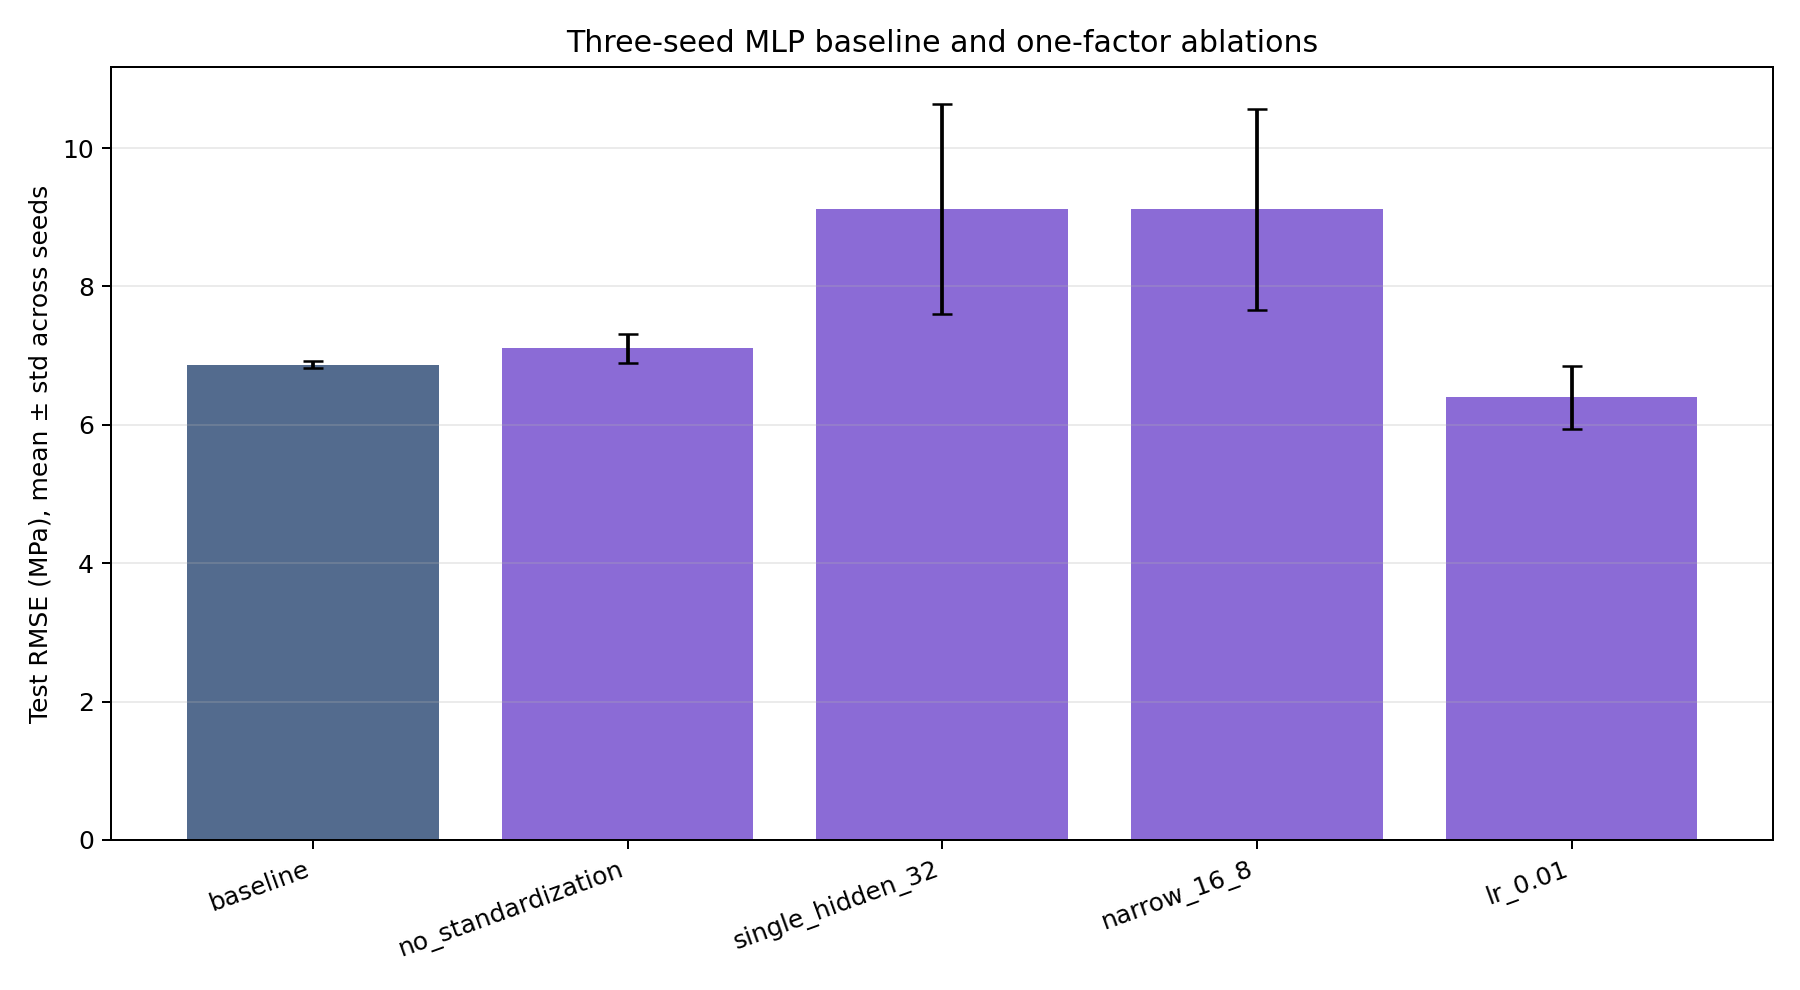
\includegraphics[width=0.485\textwidth]{images/ablation_rmse.png}
\caption{Ablation comparisons: (a) validation RMSE by epoch for seed 42; (b) mean test RMSE and standard deviation across three seeds.}
\Description{The left panel compares validation RMSE curves for five configurations at seed 42. The right panel shows mean test RMSE with standard deviation bars for three seeds; the learning-rate 0.01 configuration has the lowest mean.}
\label{fig:ablation}
\end{figure*}

\subsection{Prediction inspection}
Figure~\ref{fig:scatter} compares test predictions with measured strengths. Most points follow the ideal $y=x$ line, consistent with $R^2=0.837$, but visible deviations show that errors remain across the target range.

\begin{figure}[H]
\centering
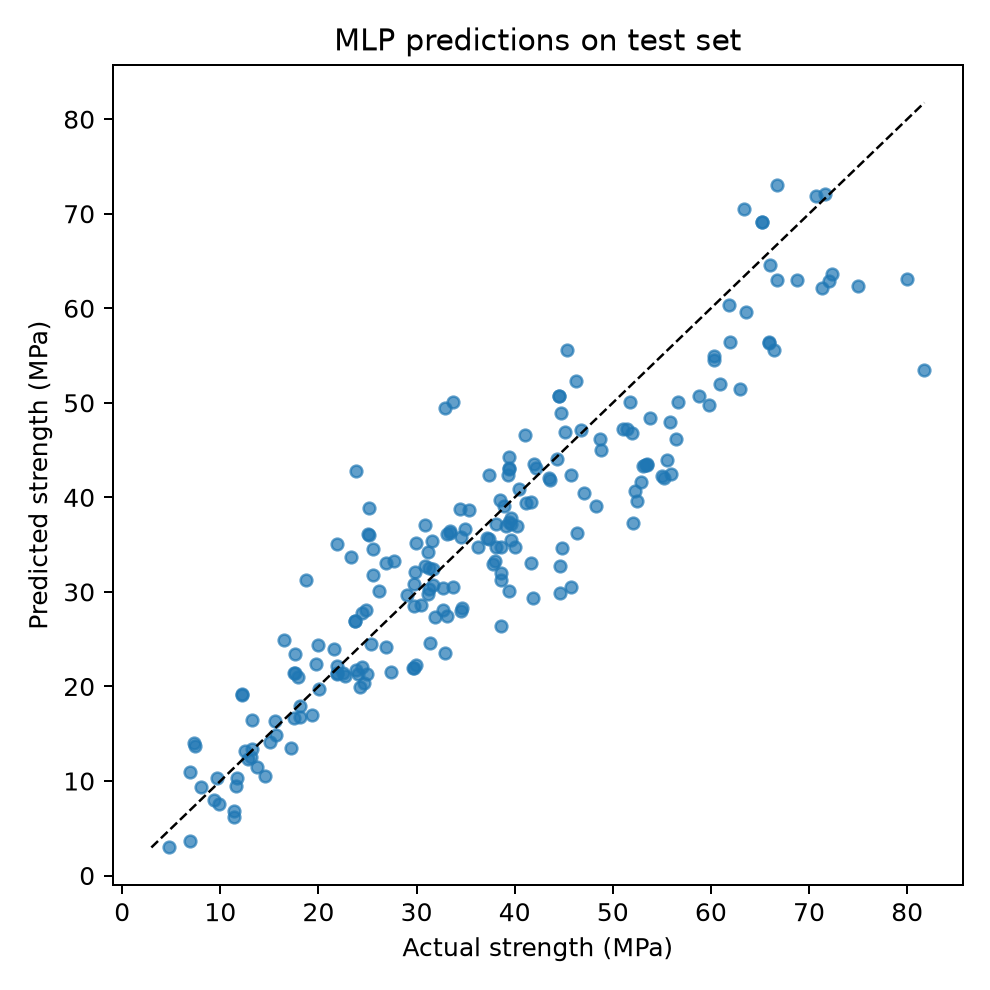
\includegraphics[width=\columnwidth]{images/prediction_scatter.png}
\caption{Measured versus predicted strength on the test split; the diagonal indicates perfect prediction.}
\Description{A scatter plot of test-set predicted strength against measured strength, with a diagonal reference line; points generally follow the line with visible errors.}
\label{fig:scatter}
\end{figure}

\subsection{Multi-seed ablation}
Table~\ref{tab:ablation} reports mean $\pm$ standard deviation across three training seeds. It addresses the effects of preprocessing, network structure, and learning rate while holding the split constant. The 0.01 learning-rate configuration has the lowest mean test RMSE (6.398 MPa) and MAE (4.680 MPa) in this small comparison. The two smaller architectures have higher mean RMSE (about 9.1 MPa) and larger variation across seeds. Removing standardization causes a modest decrease relative to baseline in this run. With only three seeds and one fixed split, these differences should be interpreted as observations for this experiment rather than universal rankings.

Figure~\ref{fig:ablation} complements the table in two ways. Panel (a) compares validation trajectories for seed 42, making convergence behavior visible; panel (b) summarizes test RMSE across all three seeds with standard-deviation bars. The validation curves show that the 0.01 learning rate descends quickly and reaches a low error, while the smaller networks converge to higher values. The error bars also show greater seed sensitivity for the smaller architectures than for the baseline.

\subsection{CPU and GPU comparison}
Table~\ref{tab:device} compares three independent 300-epoch runs per device after a five-epoch warm-up. Timing excludes the one-time data transfer, and CUDA synchronization brackets the measured interval. The CPU averages 3.065 seconds, whereas the NVIDIA GeForce MX570 averages 7.275 seconds. The CPU/GPU time ratio is 0.42, so CPU training is about 2.37 times faster for this workload. Test RMSE is similar (6.739 MPa on CPU and 6.661 MPa on GPU). Figure~\ref{fig:device-plot} visualizes the timing difference. The small dataset and network limit parallel work, so GPU launch and scheduling overhead can exceed its computational benefit; the result is specific to this machine and implementation.

\begin{table}[t]
\caption{CPU/GPU timing and test error (mean $\pm$ standard deviation, three runs).}
\label{tab:device}
\centering
\small
\begin{tabular}{lrr}
\toprule
Device & Time (s) & Test RMSE (MPa)\\
\midrule
CPU & 3.065 $\pm$ 0.049 & 6.739 $\pm$ 0.175\\
GeForce MX570 & 7.275 $\pm$ 0.254 & 6.661 $\pm$ 0.093\\
\bottomrule
\end{tabular}
\end{table}

\begin{figure}[t]
\centering
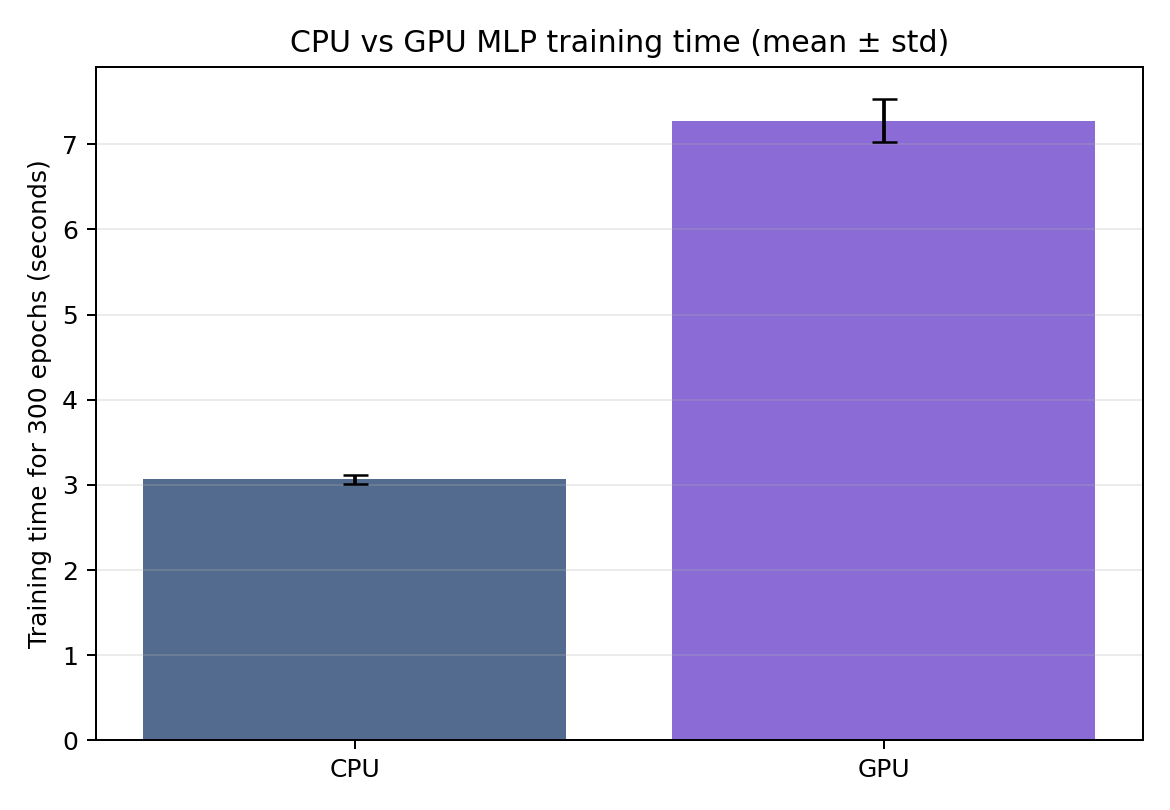
\includegraphics[width=\columnwidth]{images/cpu_gpu_training_time.png}
\caption{Mean 300-epoch training time by device; error bars show run-to-run variation.}
\Description{A bar chart showing mean training time of about 3.1 seconds for CPU and 7.3 seconds for the GeForce MX570 GPU.}
\label{fig:device-plot}
\end{figure}

\section{Conclusion}
On the fixed split, the MLP outperforms linear regression, and the multi-seed comparison suggests that architecture and learning rate affect both error and stability. The learning-rate 0.01 configuration is strongest among the five tested settings, but its result should be confirmed with more seeds or another split. CPU is faster than GPU for the small model on the available computer, despite similar test error. A useful next question is: \emph{Does the 0.01 learning rate remain advantageous when the training data are reduced or the data split is changed?}

\begin{thebibliography}{2}
\bibitem{uci}
UCI Machine Learning Repository. Concrete Compressive Strength.
\url{https://archive.ics.uci.edu/dataset/165/concrete+compressive+strength}.

\bibitem{yeh}
I.-C. Yeh. 1998. Modeling of strength of high-performance concrete using artificial neural networks. \emph{Cement and Concrete Research}. DOI: \url{https://doi.org/10.24432/C5PK67}.
\end{thebibliography}

\clearpage
\end{document}
